
%(BEGIN_QUESTION)
% Copyright 2011, Tony R. Kuphaldt, released under the Creative Commons Attribution License (v 1.0)
% This means you may do almost anything with this work of mine, so long as you give me proper credit

En ingeniør har designet følgende nivåreguleringssystem med et par split-rangede reguleringsventiler. Målet er å sikre at pumpen aldri blir ``dead-headed'' (dvs. aldri pumper mot helt stengt ventil), men alltid pumper væske {\it et sted} -- enten bort fra tanken eller i resirkulasjon tilbake til tanken:

$$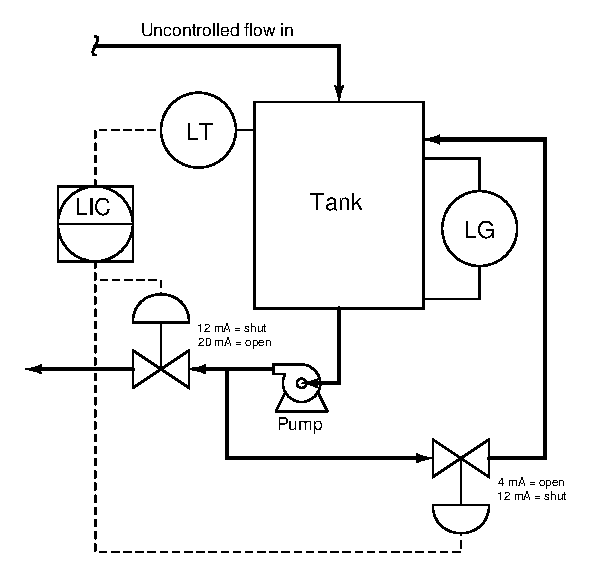
\includegraphics[width=15.5cm]{i00892x01.eps}$$

Systemet har dessverre en designfeil. Foreslå en løsning som retter feilen:

\underbar{file i00892}
%(END_QUESTION)





%(BEGIN_ANSWER)

{\bf Split-rangeringen er feil: den må være komplementær, ikke eksklusiv.} Alle svar som gir overlapp i ventilens split-range er gode svar og skal ha full uttelling.

\vskip 10pt

\noindent
{\bf Forklaring av problemet:} slik det er nå finnes fortsatt mulighet for ``dead-heading'' når regulatorutgangen er 50\%. Dessuten er nedre halvdel av regulatorområdet i praksis ubrukelig: resirkulasjonsventilen bidrar ikke til nivåregulering så lenge utgående ventil er stengt.

%(END_ANSWER)





%(BEGIN_NOTES)

{\bf Denne oppgaven er ment kun for eksamen, ikke for arbeidsark!}.

%(END_NOTES)
